\begin{wrapfigure}[8]{r}{7.5cm}
  \centering
  \vspace{-35px}
  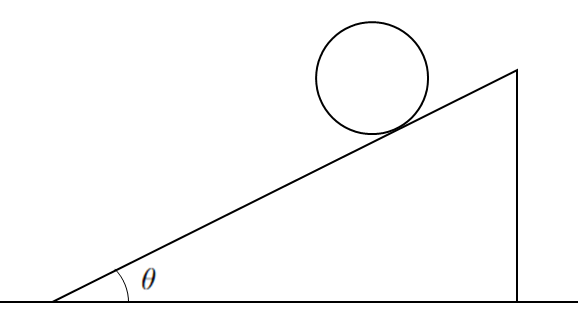
\includegraphics[width=0.35\textwidth]{images/Hinh 3.PNG}
  \begin{center}
    \figurename{ 3}
  \end{center}
\end{wrapfigure}

\vspace{-30px}
\noindent Một nêm hình tam giác có góc nghiêng $\theta$, khối lượng $M$, nằm trên mặt sàn ngang, trơn nhẵn như hình 3. Trên mặt nêm có đặt một quả cầu đồng chất khối lượng $m$, bán kính $R$. Quả cầu được thả ra từ trạng thái tĩnh và bắt đầu lăn tự do xuống dưới. Trong toàn bộ quá trình, nêm không quay. Biết gia tốc trọng trường có độ lớn $g$, giả sử hệ số ma sát nghỉ và hệ số ma sát trượt giữa quả cầu và mặt nêm đều bằng $\mu$.
\begin{enumerate}
  \item Trong trường hợp $\mu$ đủ lớn để quả cầu lăn không trượt, hãy tính:
        \begin{enumerate}
          \item[a.] Độ lớn gia tốc $a_{0}$ của nêm so với sàn.
          \item[b.] Độ lớn gia tốc $a_{C}$ của khối tâm quả cầu so với nêm.
          \item[c.] Độ lớn phản lực $N$ do mặt đất tác dụng lên nêm.
          \item[d.] Độ lớn phản lực $N_{1}$ do nêm tác dụng lên quả cầu.
          \item[e.] Giá trị nhỏ nhất $\mu_{0}$ của $\mu$ để quả cầu có thể lăn không trượt.
        \end{enumerate}
  \item Trong trường hợp $\mu$ nhỏ hơn giá trị $\mu_{0}$ tìm được và mặt nghiêng của nêm đủ dài, hãy xác định vận tốc điểm $P$ (điểm tiếp xúc giữa quả cầu và nêm) tại thời điểm $t$ kể từ khi quả cầu bắt đầu chuyển động từ trạng thái tĩnh.
\end{enumerate}